Programmet MatLabb har i stort tre delsystem:

\begin{enumerate}
\item \verb+GUI+, Det grafiska användargränssnittet
\item \Shell, eller, det inre skalet som håller centrala objekt och variabler, t.ex. aktivt recept och portionskalning.
\item \Lookup, som tillhandahåller relevanta verktyg för kommunikation med databasen.
\end{enumerate}
\verb+GUI+ ansvarar för att skriva ut data från det inre systemet på skärmen i grafisk tappning. Användaren styr även systemet genom att interagera med menyer, knappar och strängfält snarare än att ge skriftliga hänvisningar till kommandoprompten. Information presenteras enligt konceptbilderna i (figur \ref{fig:vy1} - \ref{fig:vy4}). Det grafiska gränssnittet implementeras med hjälp av biblioteket Qt och kommer delvis designas i klienten Qt Creator.

\begin{figure}[h]
  \centering
  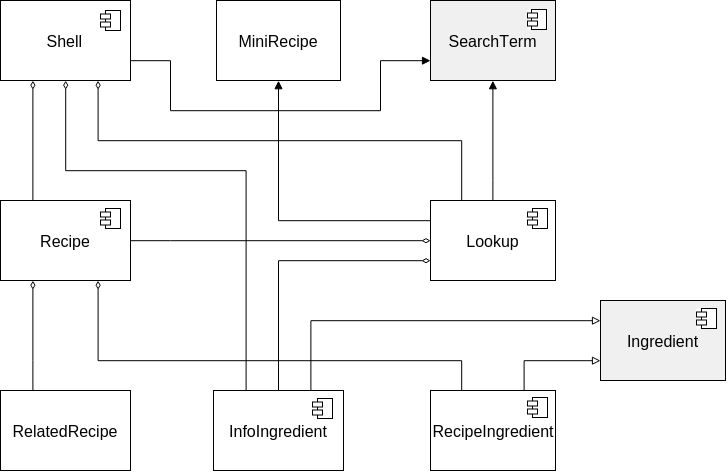
\includegraphics[scale=.4]{klass-bantad}
  \caption{Översiktsschema över MatLabbs klasser och structs. Se även figur \ref{fig:classes} (s. \pageref{fig:classes}) för närmare detaljer.}
  \label{fig:redklass}
\end{figure}

\section{Shell}
\Shell{} innehåller objekt av klasserna \Recipe{}, \InfoIngredient{} och \Lookup{} som datamedlemmar, där de två förstnämnda reflekterar det aktuella receptet och ingrediensen som vårt program interagerar med. Utåt tillhandahåller \Shell publikt endast funktioner som kan tänkas motsvara alla möjliga handlingar från användaren. Denna grupp av funktioner inkluderar, men är ej begränsade till, funktionerna listade i figur \ref{fig:tekfunklist} (s. \pageref{fig:tekfunklist}).

\begin{figure}[h]
  \caption{Funktioner för användarinputs}
  \begin{tabular}{p{5.5cm}|p{8cm}}
    \verb+addRecipe(string+) & Konstruerar ett nytt tomt \Recipe-objekt för datamedlemmen \verb+currentRecipe_+. Ett defaultargument av datatypen string existerar för att potentiellt tilldela ett namn. \\[1.2mm]
    \verb+editRecipe()+ & Kallar på \verb+currentRecipe_.editRecipe()+ för att kunna ändra på dess datamedlemmar.\\[1.2mm]
    \verb+importTxt(string)+ & Importering från textfil. Konstruerar ett nytt \Recipe-objekt och försöker fylla i dess datamedlemmar enligt en standardmodell.\\[1.2mm]
    \verb+exportTxt()+ & Kallar på \verb+currentRecipe_.exportTxt(string)+ för att exportera till .txt. Kan modifieras för att först hämta ett annat recept från databasen för exportering.\\[1.2mm]
    \verb+addIngredient(string)+ & Motsvarande \verb+addRecipe+. \\[1.2mm]
    \verb+editIngredient(string)+ &  Motsvarande \verb+addIngredient+. \\[1.2mm]
    \verb++&\\[1.2mm]
    \verb+matchRecipe(string)+ & Levererar en sträng till \verb+Lookup+-objektet för att slå i databasen för exakt matchning. \\[1.2mm]
    \verb+matchIngredient(string)+ &  Motsvarande \verb+matchRecipe+. \\[1.2mm]
    \verb+searchRecipe(cont<SearchTerm*>)+ & Levererar söktermer i en godtycklig container till \verb+Lookup+. \verb+recipeSearchResults_+ tilldelas det resultat som \verb+Lookup+ ger.  \\[1.2mm]
    \verb++&\\[1.2mm]
    \verb++& get-funktioner som används av GUI:t och returnerar relevant data. 
  \end{tabular}
  \label{fig:tekfunklist}
\end{figure}

\section{Recipe}
Objekt av klassen \Recipe{} kommer endast att existera i stabilt tillstånd som datamedlem i klassen \Shell. Nya objekt skapas antingen i samband med t.ex. funktionen \verb+addRecipe(string)+ eller byggs upp och returneras av \verb+Lookup+ som resultat av en matchning i databasen. Klassen \Recipe{} innehåller främst fullständig data om ett specifikt recept, men även funktioner för implementeringen av \Shell{}s ``användarfunktioner'', t.ex. åtkomst och redigering och för att hämta samt beräkna pris och kalorivärden. Lista över datamedlemmar i klassen \Recipe:
 
  \begin{itemize}
    \item \verb+string name_+ - \emph{Namn på receptet}
    \item \verb+string description_+ - \emph{Beskrivning/utförande}
    \item \verb+int minutesTime_+ - \emph{Tidsåtgång i minuter}
    \item \verb+cont<string> comments_+ - \emph{Kommentarer i godtycklig container}
    \item \verb+"referens" image_+ - \emph{Någon typ av referens för implentering av tillhörande bilder}
    \item \verb+double grade_+ - \emph{Betyg}
  \end{itemize}

  \begin{itemize}
    \item \verb+cont<RecipeIngredient> ingredients_+ - \emph{Ingredienser som ingår}
    \item \verb+cont<RelatedRecipe> relatedRecipes_+ - \emph{Besläktade recept}
  \end{itemize}

\subsection{MiniRecipe}
Posten \verb+MiniRecipe+ har en begränsad men viktig uppgift; objekt av denna typ representerar en nerbantad version av ett specifikt recept och existerar för att påskynda framförandet av sökresultat. När \Shell{} anropar \verb+Lookup::get_list(...)+ förväntar den sig en container innehållande \verb+MiniRecipe+s som returvärde, vilken den sparar i sin datamedlem \verb+searchResults_+.

Då en väldigt generell sökning kan tänkas generera resultat som motsvarar en majoritet av recepten i databasen, så hjälper det om programmet begränsar sig till endast den information som för stunden är relevant. Därav innehåller ett \verb+MiniRecipe+-objekt endast information om namn, tidsåtgång och betyg. Notera att inget släktskap existerar mellan \verb+MiniRecipe+ och \Recipe.

\section{Ingredient}
\Ingredient{} är en abstrakt klass ur vilken \InfoIngredient{} och \RecipeIngredient{} är härledda enligt figur \ref{fig:classes}.

\subsection{InfoIngredient}
\InfoIngredient representerar en enskild ingrediens. Utöver det gemensamma arvet så utökas \InfoIngredient med set-funktioner för att kunna redigera ingrediensens attribut.

\subsection{RecipeIngredient}
\RecipeIngredient{} representerar en enskild ingrediens som del av ett recept. Klassen utökar sitt arv med två datamedlemmar -- \verb=double amount_= och \verb=''unittype'' unit_= -- för att hantera två ytterligare funktioner: \verb+getKcal(double scaling)+ och \verb+getPrice(double scaling)+.
 
\subsection{RelatedRecipe}
\verb+RelatedRecipe+ är en struct med vissa särskilda krav, vars funktionalitet är avsedd för att agera datatyp för släktskap. Ett objekt av typen \verb+RelatedRecipe+ ska endast hänvisa släktskap med ett recept som hänvisar släktskap med det recept som objektet själv tillhör. Tanken är att strikt hålla kontroll så att inga enkelriktade släktskap ska kunna förekomma i databasen när vi väl tillför eller ändrar denna typ av information.


%HÄR BÖRJADE DU ATT ÄNDRA ERIK

\section{Lookup}
Endast ett objekt av klassen \Lookup{} existerar i programmet och då som datamedlem av \Shell. \Lookup{}s funktion är att skapa \Recipe-objekt och\InfoIngredient-objekt, samt att utföra sökningar och skapa listor av receptnamn utifrån sökningarna. Det finns även funktionalitet för att ta ut snitt union och komplement för att kunna kombinera sökresultat.

\Lookup har följande datamedlemmar
  \begin{itemize}
    \item   \verb+list_db_+ ett objekt av typen QsqlQuery som används för att söka i databasen samt att hålla datan.
    \item   \verb+ingredient_db+ enligt ovan men används endast för att skapa recept objekt.
    \item   \verb+list_pos_+ Heltal som anger hur många recept som tidigare har hämtats i databasen av \verb+query_list+
  \end{itemize}

Följande funktioner kommer användas för att göra uppslagningar,
samtliga använder \verb+Lookup+s datamedlem \verb+DB_+ och har således 
inte något returvärde. 

  \begin{itemize}
    \item   \verb+query_list+ inga parametrar, läser in 20 recept i \verb+list_db_+ och uppdaterar \verb+list_pos_+.
    \item   \verb+query_ingredient_list()+ tar en vektor med ingredienser som parameter sparar namnet på alla recept som innehåller sagda ingredienser i \verb+list_db_+.
    \item   \verb+query_ingredient_list_explicit()+ samma som ovan fast för recept som \emph{endast} innehåller sagda ingredienser i \verb+list_db_+.
    \item   \verb+query_allergy_list()+ tar en allergen som parameter och läser in alla recept innehållande sagda allergen i \verb+list_db_+.
    \item   \verb+query_price_list()+ tar ett prisintervall som parameter och läser in alla recept i givet intervall i \verb+list_db_+.
    \item   \verb+query_calory_list+ tar ett kaloriintervall som parameter och läser in alla recept i givet intervall i \verb+list_db_+.
  \end{itemize}
 

För datatillgång finns följande funktioner

\begin{itemize}
\item   \verb+get_list()+ levererar en lista över receptnamn som finns i \verb+list_db_+
\item   \verb+get_recipie()+ tar ett receptnamn som parameter och returnerar ett objekt av typen \verb+recipe+.
\item   \verb+get_info_ingredient()+ tar ett ingrediensnamn som parameter och returnerar ett objekt av typen \verb+info_ingredient+.
\item   \verb+get_recipe_ingredient()+ hjälpfunktion till \verb+get_recipe+.
\end{itemize}

\Lookup kommer alltså inte att klara av alla olika kombinationer av sökningar på egen hand då detta skulle vara komplicerat att implementera utan kommer istället utgå från de sökningar som finns och sedan med hjälp av följande funktioner slå ihop listor för att nå fram till det resultat som önskas. Samtliga tar två listor som parametrar och returnerar en sammanslagen lista.

\begin{itemize}
\item   \verb+union()+ returnerar ihop unionen av två listor.
\item   \verb+intersect()+ returnerar snittet av två listor.
\item   \verb+complement()+ returnerar två listors komplement.
\end{itemize}


\section{EditDB}

\verb+EditDB+ är den klass som används för att skriva data till databasen. Den
skall kunna hantera tilläggning och borttagning av ingredienser samt recept. Den
skall även kunna Lägga till kommentarer till ett recept samt lägga till redskap
i databasen.

För att klara detta använder den sig av följande funktioner för insättning

%Lista över funktioner för tillägning
\begin{itemize}
\item \verb+add_recipe()+ Tar emot ett \verb+recipie+-objekt som parameter och updaterar
  databasen ifall receptet fanns sedan innan eller lägger till ifall det inte
  fanns.

\item \verb+add_ingredient()+ Tar emot ett \verb+ingredient+-objekt som parameter
  och updatera databasen om ingrediensen fann sedan innan eller lägger till om
  det inte fanns.

\item \verb+add_comment()+ Tar emot ett receptnamn och en kommentar som
  parametrar och lägger till kommentaren till motsvarande recept

\item \verb+add_tool()+ Tar emot ett namn på ett redskap och lägger till det i
  databasen.

\end{itemize}


Och följande funktioner för borttagning

%Lista över funktioner för borttagning.
\begin{itemize}

\item \verb+remove_recipe()+ Tar emot ett receptnamn som parameter och raderar
  motsvarande recept ur databasen.

\item \verb+remove_ingredient()+ Tar emot ett ingrediensnamn som parameter och
  raderar motsvarande ingrediens ur databasen.

\item \verb+remove_tool()+ Tar emot ett redskapsnamn och tar bort motsvarande
  redskap i databasen.

\item \verb+remove_comment()+ Tar emot ett kommentars-id och tar bort
  motsvarande kommentar.
  
\end{itemize}

Endast en datamedlem finns och är av typen QsqlQuery vid namn \verb+db_+ och
används för att sköta kontakten med databasen




%HÄR SLUTADE DU SKRIVA ERIK

\begin{figure}[h]
\centering
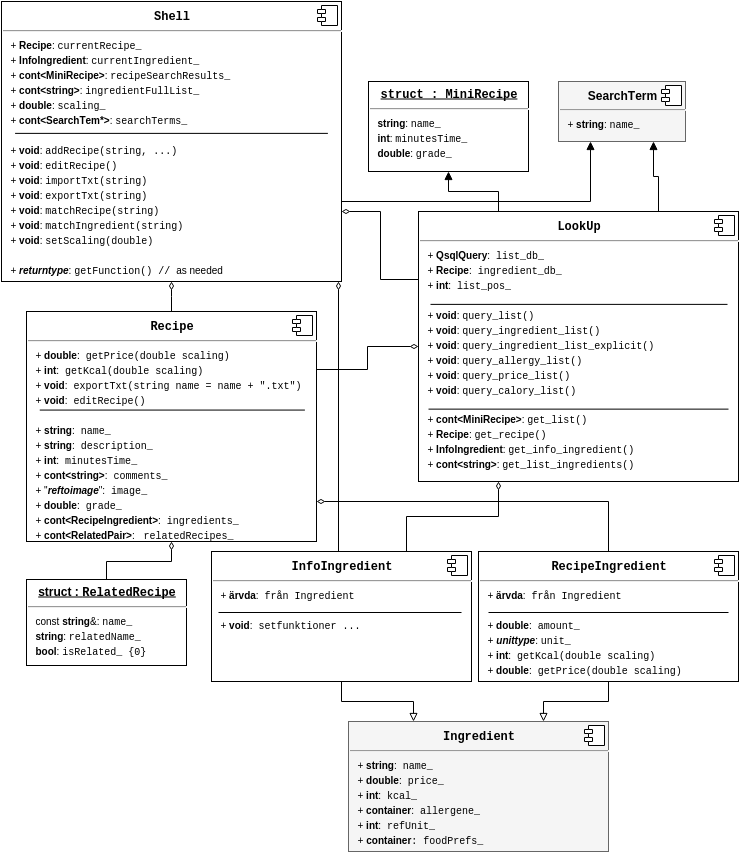
\includegraphics[width=16cm]{klass-schema.png}
\caption{Klass-schema}
\label{fig:classes}
\end{figure}


